\chapter{Theoretical Background} % Main chapter title
\label{chap:Chapter2} % For referencing the chapter elsewhere, use \ref{Chapter1} 
\epigraph{''Let no one ignorant of geometry enter” }{\textit{Plato}}

O χώρος των \hyperref[abbr:WSN]{WSN} έχει και αυτός τα τελευταία χρόνια υψηλό ερευνητικό ενδιαφέρον.
Θα μπορούσε να πει κανείς - λόγο το ότι αποτελεί ένα πιο γενικό κλάδο - περισσότερο από ότι αυτό των 
drones. Συνεπώς θα μεταφερθούμε σε πρώτο επίπεδο στο πιο γενικό φάσμα, αυτό των \hyperref[abbr:WSN]{WSN} 
για να προσεγγίσουμε το localization problem. 

Όταν μιλάμε για \hyperref[abbr:WSN]{WSN}, αναφερόμαστε σε αυτόνομα ηλεκτρονικά συστήματα, χωρικά διασκορπισμένα σε ένα πεδίο - τα οποία συχνά περιλαμβάνουν
αισθητήρες και επικοινωνούν με τα γειτονικά τους ή σταθμούς βάσης για να μεταφέρουν πληροφορία \cite{wsn-wikipedia}.

Το καθένα από αυτά τα μεμονωμένα συστήματα ονομάζεται \textbf{Node}. Ενώ για το κάθε μεμονωμένο node 
μπορεί να έχουμε στην διάθεση μας location information ή όχι. 
Μία πρώτη σκέψη θα ήταν κάθε Node ενός συστήματος αισθητήρων να περιλαμβάνει \hyperref[abbr:GPS]{GPS} ώστε να γνωρίζουμε 
την θέση του. Αυτό μπορεί γρήγορα να καταρριφθεί σαν σκέψη, αν αναλογιστούμε αρχικά ότι το Global Navigation Satellite System (\hyperref[abbr:GNSS]{GNSS})
δεν είναι διαθέσιμο σε κάθε περιβάλλον λειτουργίας (π.χ. εσωτερικούς χώρους), όπως επίσης μπορεί να μην είναι δυνατή η χρήση του σε όλους τους κόμβους
ενός συστήματος, λόγο περιορισμών όπως το κόστος, μέγεθος του Node και energy consumption.   

\begin{table}[H]
    \caption{Nodes' names definitions}
    \label{tab:nodes-names-definition}
	\centering
	\resizebox{1\textwidth}{!}{
		\begin{tabular}{ll}
			\toprule
			\textbf{Node name} & \textbf{Definition}  \\
			\midrule
				Unknown/Free/Dumb/Non-anchors & Their position is unknown \\
				Beacons/Anchors/Landmarks & Nodes with known location information \\
				Settled & Initial unknown nodes with estimated position \\
			\bottomrule
		\end{tabular}
	}
\end{table}

Στην υπάρχουσα βιβλιογραφία \cite{wsn-Localization-systems} \cite{wsn-Localization-techniques} βρίσκουμε ότι
Nodes των οποίων η θέση είναι γνωστή ή άμεσα υπολογίσιμη, συχνά ονομάζονται \textbf{Beacons}. Πληροφορία σχετικά με την θέση αυτών
των Nodes είναι γνωστή, είτε γιατί έχουν τοποθετηθεί από εμάς σε προκαθορισμένες θέσεις, είτε μέσου ενός εξωτερικού συστήματος
όπως το \hyperref[abbr:GPS]{GPS}.
Αντίθετα κόμβοι για τους οποίους δεν έχουμε αρχικά πληροφορία της θέσης τους, ονομάζονται \textbf{Non-anchors}.
Άλλος ένας σημαντικός ορισμός, που θα πρέπει να αναφερθεί είναι ότι συχνά ονομάζουμε \textbf{Settle} nodes, 
αυτά τα οποία αρχικά δεν γνωρίζαμε την θέση τους αλλά στην συνέχεια την εκτιμήσαμε.
Στο table \ref{tab:nodes-names-definition} παρουσιάζονται συνοπτικά τα διάφορα ονόματα που έχουν δοθεί ανά 
καιρούς για το κάθε τύπο node.

Σκοπός ενός localization system είναι, με χρήση της γνώσης που έχουμε για τα beacon nodes να εκτιμήσουμε
την θέση όσο περισσότερων unknown nodes ώστε να τα μετατρέψουμε σε settled nodes και η εκτίμηση της κάθε
θέσης να είναι με όσο το δυνατόν μικρότερο error απόκλισης. 

\begin{figure} [H]
	\centering
	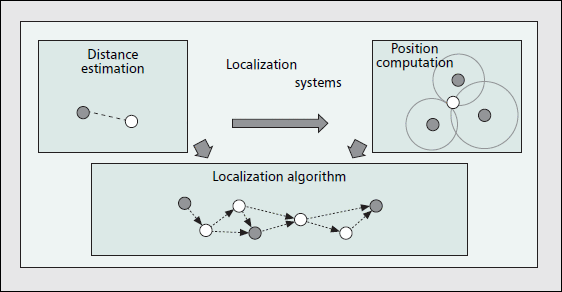
\includegraphics[scale=0.5]{Images/Theoretical-Background/localization-systems-components.png}
	\decoRule
	\caption[Localization System components]{Localization System components based on \cite{wsn-Localization-systems} (\href{https://ieeexplore.ieee.org/document/4407221}{URL})}
	\label{fig:Localization-Systems-components}
\end{figure}

Οι συγγραφείς του \cite{wsn-Localization-systems} επιχειρούν να χωρίσουν ένα localization system, ώστε 
αυτό να αποτελείται από τρία διακριτά components. Πρώτο μπορεί να θεωρηθεί αυτό του \textbf{Distance/Angle Estimation}, 
που σκοπό έχει να υπολογίσει την απόσταση ή γωνία που έχουν δύο nodes του συστήματος μεταξύ τους.
Η πληροφορία που θα παραχθεί από αυτό το component θα χρησιμοποιηθεί στα άλλα μέρη του συστήματος.
Στην συνέχεια υπάρχει το \textbf{Position Computation}, δουλειά του οποίου είναι να υπολογίσει την θέση ενός
node με βάση την γνώση που έχουμε για τα beacons και την πληροφορία που λάβαμε από το πρώτο component.
Ενώ τέλος είναι το κύριο μέρος του συστήματος, με όνομα \textbf{Localization Algorithm} και ουσιαστικά είναι
ο προκαθορισμένος τρόπος που θα ακολουθηθεί για να υπολογιστεί η θέση των unknown nodes με βάση όλες τις 
πληροφορίες που έχουμε.
Στο figure \ref{fig:Localization-Systems-components} δίνεται η απεικόνιση που έδωσαν οι συγγραφείς του 
\cite{wsn-Localization-systems} για να εξηγήσουν το παραπάνω. Ενώ στο figure \ref{fig:Localization-system}
έχει γίνει μία προσπάθεια να κατηγοριοποιηθούν τα κομμάτια καθώς και τεχνικές των Localization Systems,
με βάση τα \cite{wsn-Localization-systems} \cite{wsn-Localization-techniques} και αναλύονται στην συνέχεια
του κεφαλαίου.

\begin{figure} [H]
	\tikzset{
		basic/.style  = {draw, text width=2cm, font=\sffamily},
		root/.style   = {basic, thin, align=center, fill=white, text width=5cm},
		level 1/.style = {sibling distance=16em, level distance=5em},
		level-2/.style = {basic, thin, align=center, fill=white, text width=5.5cm},
		level-31/.style = {basic, thin, align=center, fill=white, text width=2cm},
		level-32/.style = {basic, thin, align=center, fill=white, text width=2.8cm},
		level-33/.style = {basic, thin, align=center, fill=white, text width=5cm},
		level-4/.style = {basic, thin, align=center, fill=white, text width=4.5cm},
		level-42/.style = {basic, thin, align=center, fill=white, text width=4.8cm},
		edge from parent/.style={->,solid,black,thick,draw}, 
		edge from parent path={(\tikzparentnode.south) -- (\tikzchildnode.north)},
		>=latex, node distance=1.5cm, edge from parent fork down
	}
	\centering
	\resizebox{1\textwidth}{!}{
		\begin{tikzpicture}[]
			\node[root] {\textbf{Localization Systems}}
				child {node[level-2] (c1) {\textbf{Distance/Angle Estimation}}}
				child {node[level-2] (c2) {\textbf{Position Computation}}}
				child {node[level-2] (c3) {\textbf{Localization Algorithm}}};
			
			% -----------------------------------------------------------------------------
			% Distance/Angle
			\node [level-31, below of = c1, xshift=-25pt] (c11) {Distance};
				\node [level-4, below of = c11, xshift=50pt] (c111) {Received Signal Strength};
				\node [level-4, below of = c111] (c112) {Lighthouse approach};
				\node [level-4, below of = c112] (c113) {Propagation time based measurements};
					\node [level-42, below of = c113, xshift=30pt] (c1131) {One-way propagation time};
					\node [level-42, below of = c1131] (c1132) {Roundtrip propagation time};
					\node [level-42, below of = c1132] (c1133) {Time Difference of Arrival};
					\foreach \value in {1,2,3} \draw[->] (c113.197) |- (c113\value.west);
				\foreach \value in {1,2,3} \draw[->] (c11.195) |- (c11\value.west);

			\node [level-31, below of = c1133, xshift=-80pt] (c12) {Angle};
				\node [level-4, below of = c12, xshift=70pt] (c121) {Receiver Antenna Amplitude response};
				\node [level-4, below of = c121] (c122) {Receiver antenna Phase response};
				\foreach \value in {1,2} \draw[->] (c12.210) |- (c12\value.west);
			\foreach \value in {1,2}   \draw[->] (c1.188) |- (c1\value.west);
			
			% Position Computation
			\node [level-32, below of = c2, xshift=25pt] (c21) {Trilateration};
			\node [level-32, below of = c21] (c22) {Bounding box};
			\node [level-32, below of = c22] (c23) {Triangulation};
			\node [level-32, below of = c23] (c24) {Multilateration};
			\node [level-32, below of = c24] (c25) {Probabilistic approaches};
			\node [level-32, below of = c25] (c26) {Central position};
			\foreach \value in {1,...,6} \draw[->] (c2.196) |- (c2\value.west);

			% Localization Algorithm
			\node [level-33, below of = c3, xshift=10pt] (c31) {Distributed/Centralized \\ Position Computation};
			\node [level-33, below of = c31] (c32) {With/Without Infrastructure};
			\node [level-33, below of = c32] (c33) {Relative/Absolute Positioning};
			\node [level-33, below of = c33] (c34) {Indoor/Outdoor scenarios};
			\node [level-33, below of = c34] (c35) {One-hop/Multihop};
			\foreach \value in {1,...,5} \draw[->] (c3.187) |- (c3\value.west);
		\end{tikzpicture}
	}
	\decoRule
	\caption[Localization-system-overview]{Localization system overview}
	\label{fig:Localization-system}
\end{figure}


%----------------------------------------------------------------------------------------
%	SECTION 1
%----------------------------------------------------------------------------------------
\section{Distance/Angle Estimation} \label{sec:Chapter2-1} 

\subsection{Distance}\label{sec:Chapter2-1-1}

Θα ξεκινήσουμε με μία σύντομη ανάλυση των τεχνικών εκτίμησης της απόστασης μεταξύ δύο nodes
που χρησιμοποιούνται ήδη. 

%----------------------------------------------------------------------
\subsubsection{Received Signal Strength}
Η πρώτη τεχνική η οποία έχει χρησιμοποιηθεί για τον υπολογισμό απόστασης στα 
\hyperref[abbr:WSN]{WSN} είναι αυτή με όνομα Received Signal Strength Indicator
(\hyperref[abbr:RSSI]{RSSI}) και έχει ως αρχή, την χρήση της έντασης ενός 
σήματος που λαμβάνουμε στον δέκτη, ως τρόπο υπολογισμού της απόστασης
του πομπό από αυτόν. Στον ελεύθερο χώρο η λαμβανόμενη ισχύς που ανιχνεύει ο πομπός
$P_r(d)$ μπορεί να περιγραφεί από την σχέση (\ref{eq:signal-strength}) \cite{wsn-Localization-techniques}.

\begin{align}
	P_r(d)=\frac{P_tG_tG_r\lambda^2}{(4\pi)^2d^2} \label{eq:signal-strength}
\end{align}

Όπου $P_t$ είναι η ισχύς που στέλνει ο πομπός, $G_t$ είναι το gain της κεραίας του
πομπού, $G_r$ το gain της κεραίας του δέκτη, λ είναι το μήκος κύματος του σήματος
το οποίο μεταδίδουμε και d η απόσταση του πομπού από τον δέκτη. Αν θεωρήσουμε ότι 
τα $G_t$, $G_r$ και λ είναι μη μεταβλητές τιμές - με $C_f = \frac{G_tG_r\lambda^2}{(4\pi)^2}$ - τότε μπορούμε να καταλήξουμε
στην (\ref{eq:signal-strength-simple}) \cite{rssi-simple-formula}

\begin{align}
	P_r(d)=C_f\frac{P_t}{d^2} \label{eq:signal-strength-simple}
\end{align}

Αυτό που μπορούμε να δούμε από την παραπάνω σχέση είναι ότι, ιδανικά στον ελεύθερο 
χώρο σε Line of Sight (\hyperref[abbr:LoS]{LoS}) μετάδοση -
η ισχύς του σήματος που λαμβάνει ο πομπός εξαρτάται από το αντίστροφο τετράγωνο της
απόστασης των δύο nodes. Το figure \ref{fig:Ideal-RSSI-over-distance} περιγράφει 
σχηματικά αυτήν την εξάρτηση. 

%-------------------------------------------

\begin{figure} [H]
	\centering
	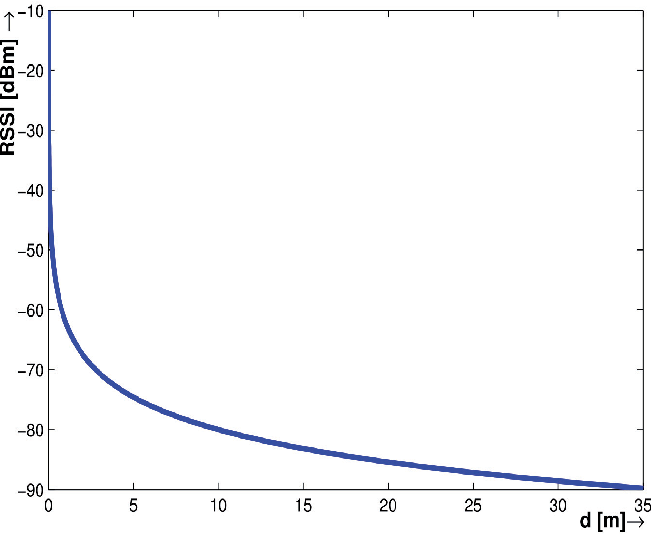
\includegraphics[scale=0.32]{Images/Theoretical-Background/Ideal-RSSI-over-distance.png}
	\decoRule
	\caption[Ideal RSSI over distance]{Ideal RSSI over distance based on \cite{ideal-rssi-model}}
	\label{fig:Ideal-RSSI-over-distance}
\end{figure}

Αυτή η μέθοδος παρόλο που είναι αρκετά δημοφιλής και οικονομική για τον υπολογισμό της απόστασης
- λόγω του ότι δεν απαιτεί επιπλέον αισθητήρες - σε πραγματικές 
συνθήκες αντιμετωπίζει αρκετά προβλήματα, καθώς οι μετρήσεις μπορούν να επηρεαστούν από θόρυβο,
ανακλάσεις του σήματος, διαθλάσεις, δυναμικά περιβάλλοντα ή εμπόδια σε αυτά, ή ακόμα και errors στο hardware 
\cite{wsn-Localization-systems} \cite{ideal-rssi-model}.
Σε ένα βαθμό μπορεί να βελτιωθεί η απόδοση με στατικό ή δυναμικό calibration του συστήματος 
όμως μέχρι τώρα δεν χρησιμοποιείται για εκτίμηση απόστασης σε εφαρμογές όπου nodes έχουν μεγάλη
απόσταση μεταξύ τους ή μας ενδιαφέρει να έχουμε μεγάλη ακρίβεια προσέγγισης της απόστασης \cite{ideal-rssi-model}.

%----------------------------------------------------------------------
\subsubsection{Propagation Time}
Σε αυτήν την κατηγορία εκτίμησης απόστασης μεταξύ nodes - η οποία βασίζεται σε χρονικές μετρήσεις της διάδοσης του σήματος
- κατά κύριο λόγο χρησιμοποιούνται δύο βασικές τεχνικές, η Time of Arrival (\hyperref[abbr:ToA]{ToA}) και η Time 
Difference of Arrival (\hyperref[abbr:TDoA]{TDoA}) \cite{wsn-Localization-systems}. 

\begin{figure} [H]
    \centering
    % -----------------
    \begin{minipage}{.5\textwidth}
      \centering
      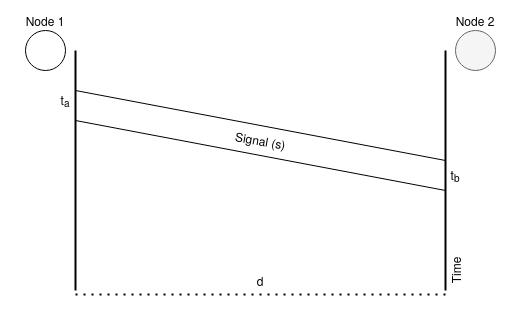
\includegraphics[width=\linewidth]{../Photos/toa-oneway.png}
      {(a) One-way}
    \end{minipage}%
    % -----------------
    \begin{minipage}{.5\textwidth}
      \centering
      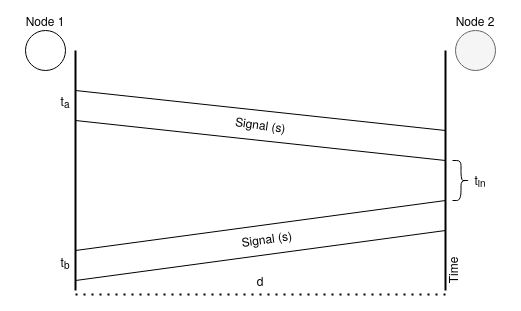
\includegraphics[width=\linewidth]{../Photos/toa-roundtrip.png}
      {(b) Roundtrip}
    \end{minipage}
    \hfill \break
    \decoRule
    \caption[Time of Arrival cases]{Time of Arrival cases}
    \label{fig:Time-of-Arrival-cases}
\end{figure}

Θα ξεκινήσουμε με μία σύντομη περιγραφή της \hyperref[abbr:ToA]{ToA}. Από την κινηματική γνωρίζουμε την 
σχέση (\ref{eq:speed}), η οποία συσχετίζει την ταχύτητα κίνησης ενός σώματος V ως το πηλίκο της μεταβολής
της θέσης $\mathrm{d}s$ - που έκανε το σώμα, προς τον χρόνο $\mathrm{d}t$ που χρειάστηκε για να πραγματοποιηθεί η μεταβολή \cite{Kinematics}.

\begin{align}
	V=&\frac{\mathrm{d}s}{\mathrm{d}t} \label{eq:speed} \\
	d=&s(t_b-t_a) \label{eq:distance}
\end{align}

Αξιοποιώντας την (\ref{eq:speed}) ως αρχή, μπορούμε να καταλήξουμε στην (\ref{eq:distance}) για να εκτιμήσουμε
την απόσταση d που βρίσκονται δύο nodes μεταξύ τους, αν ένα κύμα κινείται με ταχύτητα $s$ και χρειάστηκε 
χρόνο $t$ για να μεταδοθεί από το ένα node στο άλλο. Στο figure \ref{fig:Time-of-Arrival-cases} (a) απεικονίζεται
σχηματικά αυτό, όπου $t=t_b-t_a$ με $t_b$ η χρονική στιγμή που φτάνει το κύμα στο receiver και $t_a$
η χρονική στιγμή η οποία ξεκινάει από τον transmitter. Σε περίπτωση που μιλάμε για Radio Frequency 
(\hyperref[abbr:RF]{RF}) η ταχύτητα μετάδοσης του κύματος είναι ίση με την ταχύτητα μετάδοσης του φωτός $c_o$.
Με βάση αυτό, μπορούμε εύκολα να καταλάβουμε ότι για να έχουμε ακριβή αποτελέσματα είναι αρκετά σημαντικό
τα clocks των δύο nodes να είναι απόλυτα συγχρονισμένα, πράγμα που
απαιτεί να κάνουμε το συνολικό σύστημα αρκετά πιο πολύπλοκο σχεδιαστικά \cite{wsn-Localization-systems} \cite{wsn-Localization-techniques}.

Μπορούμε να το παρακάμψουμε αυτό, με το να γίνει η μέτρηση σε roundtrip μετάδοση, figure \ref{fig:Time-of-Arrival-cases} (b).
Σε αυτήν την περίπτωση το ένα node στέλνει ένα σήμα, και μόλις το λάβει ένα γειτονικό node, απαντάει πίσω στο πρώτο. 
Με αυτόν τον τρόπο η μέτρηση του χρόνου εκκίνησης και άφιξης του σήματος γίνονται στο ίδιο node - 
άρα δεν χρειάζεται συγχρονισμός, και η πραγματική απόσταση είναι η μισή από αυτή που θα υπολογιστεί. Ο κύριος παράγοντας
σφάλματος σε αυτή την μέθοδο είναι ο υπολογισμός του χρόνου που χρειάστηκε το δεύτερο node για να διαχειριστεί
το σήμα που έλαβε και να απαντήσει, αυτό το internal delay μπορεί να είναι είτε γνωστό από 
ένα a priori calibration, είτε μπορεί να μετριέται και να στέλνεται μαζί με το σήμα απάντησης - ώστε να αφαιρείται
από τον χρόνο μετάδοσης του κύματος \cite{wsn-Localization-techniques}.

Όσον αφορά την τεχνική \hyperref[abbr:TDoA]{TDoA}



%----------------------------------------------------------------------
\subsubsection{Lighthouse}

%----------------------------------------------------------------------
\subsection{Angle}\label{sec:Chapter2-1-1}

%----------------------------------------------------------------------------------------
%	SECTION 2
%----------------------------------------------------------------------------------------
\section{Position Computation} \label{sec:Chapter2-2} 

%----------------------------------------------------------------------------------------
%	SECTION 3
%----------------------------------------------------------------------------------------
\section{Localization Algorithm} \label{sec:Chapter2-3} 

